\section{RF Antennas}
Generally, an antenna is a system which allows to couple electromagnetic energy from a circuit into free space. It uses the benefit that an oscillating magnetic field generates an oscillating electric field and vise versa.

\subsection{Antenna Parameters}

\begin{minipage}{10cm}
\begin{itemize}
	\item \textbf{Impedance Matching:} To transfer the maximum energy from the transmission line over the antenna to free space folowing condition should be satisfied:
	\begin{equation}
	Z_{ant} = Z^*_{TL} 
	\end{equation}
	\item \textbf{Radiation Pattern:} Defines how the electromagnetic energy radiated by the antenna is spatially distributed in free space. (Doughnut plots)\\ It is the normalized radiation intensity in a polar plot. It is usually given in dB: \\
	$F_{dB}(\phi,\theta)=10log_{10}F(\phi,\theta)$
	\item \textbf{Radiation Efficiency:} Defines the ratio between the radiated energy and the energy applied to the antenna system.
	\item \textbf{Bandwidth:} Usually, the bandwidth is defined as the frequency range where the radiated power is up to 10dB below the maximum radiated power ( $1<VSWR<1.5$)
	\item \textbf{Near Field:} $\lambda < r < 4$	\hspace{2cm} \textbf{Far Field:} $ r > 10\cdot \lambda$
	\item \textbf{Reciprocity:} An antenna receives signals as good as it can transmit them.

\end{itemize}
\end{minipage}
\begin{minipage}{8cm}
	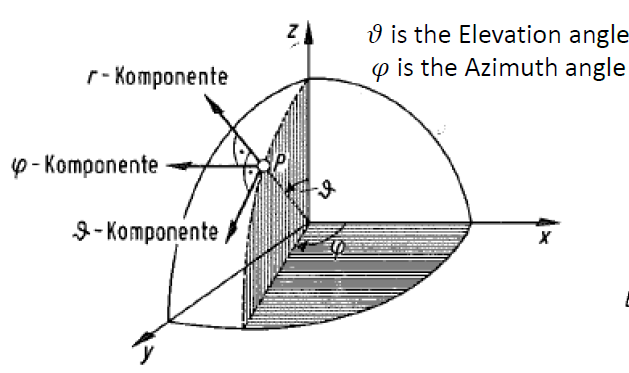
\includegraphics[width=1\textwidth]{./images/Antenna_Pattern.png}\\
\end{minipage}

\begin{tabular}{|l|c|c|}
	\hline \textbf{Description} & \textbf{Equation} & \textbf{Hertzian Dipole}\\
	\hline Impedance of free space (Far field only) & $Z_0 =\frac{E_\theta}{H_\phi} = \sqrt{\frac{\epsilon_0}{\mu_0}} \approx 377 \Omega$ & \\
	\hline Time averaged radiated Power & $S(r,\phi,\theta)=\int_{0}^{T}\vec{E}\hspace{0.1cm} x\hspace{0.1cm} \vec{H}dt $ & $Z_0 \frac{I_0^2}{r}(\frac{d}{\lambda})^2 \hspace{0.1cm} sin^2 \theta$ \\
	\hline Total radiated Power & $ P_s=\int_{\phi}^{}\int_{\theta}^{}S(r,\phi,\theta)\cdot r^2 sin\theta \hspace{0.1cm} d\theta\hspace{0.1cm} d\phi$ & $Z_0 I_0^2 \frac{\pi}{12}(\frac{d}{\lambda})^2$   \\
	\hline Normalized Radiation Intensity & $ F(\phi,\theta)=\frac{S(r,\phi,\theta)}{max[S(r,\phi,\theta)]}$ & $sin^2 \theta$\\
	\hline Power density of Isotropic Antenna (fictional) & $ S_i = \frac{P_s}{4\pi r^2}$ & \\
	\hline Directivity (in a preferred direction) & $ D = \frac{max[S(r,\phi,\theta)]}{S_i}$ & $\approx 1.5 $ depends on the length\\
	\hline Radiation Resistance & $ R_{rad} = \frac{2P_{rad}}{I_0^2}$ & \\
	\hline Radiation Power & $ P_{rad} = 0.5 \cdot I_0^2 \cdot R_{rad} $ & \\ 
	\hline Antenna (ohmic) losses & $ P_{loss} = 0.5 \cdot I_0^2 \cdot R_{loss} $ & \\ 
	\hline Radiation Efficiency & $ \eta = \frac{P_{rad}}{P_{P_tot}}$ & \\
	\hline Antenna Gain & $G = \eta \cdot D $ & \\
	\hline Equivalent Isotropic Radiated Power & $EIRP = G \cdot P_s$ & \\
	\hline Antenna Impedance & $ Z_{ant} = R_{loss}+R{rad} +jX $ & \\
	\hline Reflection Factor & $\Gamma = \frac{Z_{Ant}- Z_{TL}}{Z_{Ant} + Z_{TL}}$ & \\
	\hline Voltage Standing Wave Ratio & $ VSWR = \frac{1+\Gamma}{1-\Gamma} > 1$ & \\
	\hline Effective Antenna Area & $ A_{eff,RX} = \frac{P_{RX}}{S(r,\phi,\theta)} = \frac{\lambda^2 D_{RX}}{4\pi} $ & \\
	\hline Ratio between transmitted and received power & $ P_{RX} = P_{TX}\cdot G_{TX}\cdot G_{RX}\cdot (\frac{\lambda}{4 \pi R})^2 $ & R = Distance between Antennas\\
	\hline Free Space Path Loss & $ FSPL = 20log_{10} \frac{4\pi R}{\lambda}$ & $\lambda = \frac{c}{f}$ \\
	\hline 
\end{tabular} 



\newpage
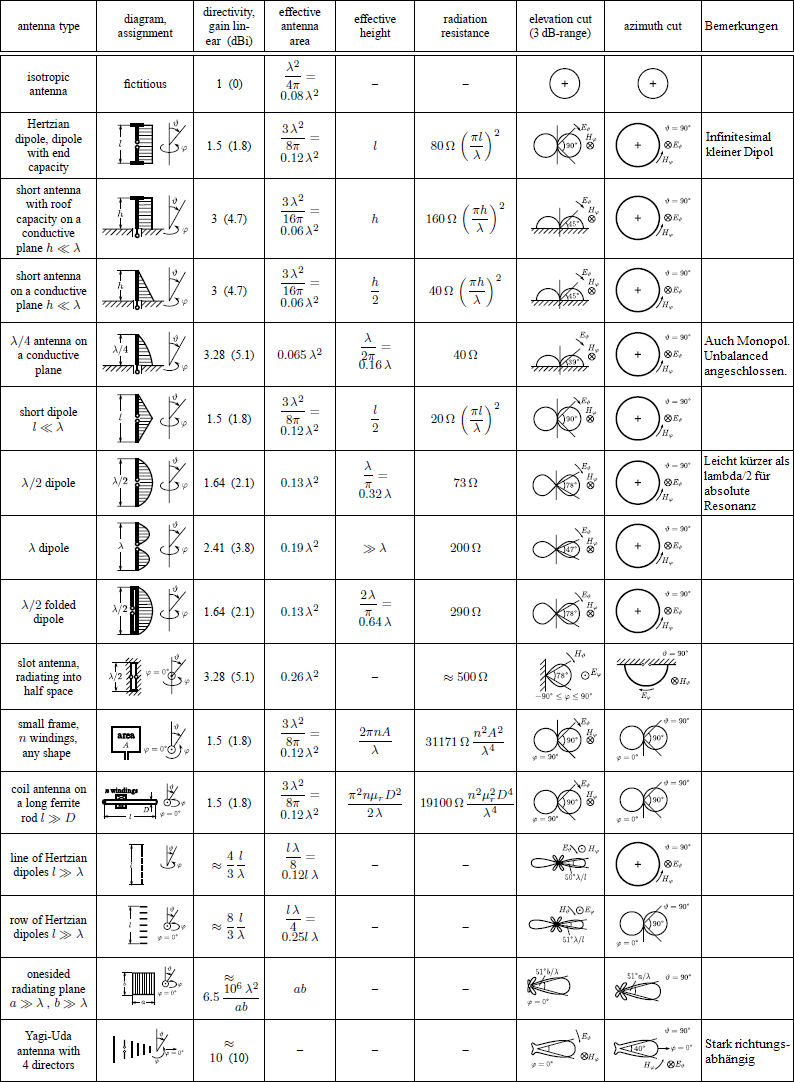
\includegraphics[width=1\textwidth]{./images/antennas-overview.png}\\